\documentclass[a4paper, 11pt]{scrartcl}

\usepackage[utf8]{inputenc}
\usepackage[ngerman]{babel}

\usepackage{mathptmx}
\renewcommand{\familydefault}{\sfdefault}

% Settings for page geometry
\usepackage[left=2.5cm, right=2.5cm, top=2.5cm, bottom=2.5cm]{geometry}
\usepackage[onehalfspacing]{setspace}

% ETC Packages
\usepackage{amsmath}
\usepackage{amssymb}
\usepackage{graphicx}
\usepackage{xcolor}
\usepackage{floatflt,epsfig}
\usepackage{scrlayer-scrpage}
\usepackage{hyperref}
\usepackage{float}
\usepackage{sectsty}

\usepackage{xcolor}
\usepackage{floatflt,epsfig}
\usepackage[framemethod=tikz]{mdframed}
% \usepackage[fleqn]{amsmath}
\usepackage{listings}
\usepackage{color}
%\usepackage{minted}

\mdfsetup{
    skipabove=\topskip ,
    skipbelow=\topskip ,
    innertopmargin=-0.2cm,
    innerbottommargin=-0.2cm,
    innerleftmargin=0cm
}

\definecolor{dkgreen}{rgb}{0,0.6,0} % comment style
\definecolor{gray}{rgb}{0.5,0.5,0.5}
\definecolor{mauve}{rgb}{0.58,0,0.82} 
\definecolor{BBS}{RGB}{0,169,164} % Teal color of BBS logo
\definecolor{ssh}{RGB}{22,198,12} % bash connection / user
\definecolor{path}{RGB}{59,120,184} % Bash current working directory
\definecolor{bbg}{RGB}{50,50,50} % Bash Background
\definecolor{cfg}{RGB}{58,150,221} % Bash Background

\lstset{ % defining an environment for bash code
    escapeinside={<@}{@>},
    aboveskip=3mm,
    belowskip=3mm,
    showstringspaces=false,
    columns=flexible,
    basicstyle={\small\ttfamily\color{white}},
    numbers=none,
    numberstyle=\tiny\color{white},
    commentstyle=\color{dkgreen},
    stringstyle=\color{blue},
    breaklines=true,
    breakatwhitespace=true,
    tabsize=3,
    morekeywords={
        sudo, apt, git, ufw
    }
}

% Define colors for headings of different parts of the documentation
\sectionfont{\color{BBS}}
\subsectionfont{\color{BBS}}
\subsubsectionfont{\color{BBS}}

\begin{document}
% \begin{spacing}{1.3}
\thispagestyle{empty}
\ihead{
    \begin{footnotesize}
        Deployment einer Rest API
    \end{footnotesize}
}
\chead{
    \begin{footnotesize}
        Lernfeld 9: Netzwerke und Dienste bereitstellen
    \end{footnotesize}
}
\ohead{
    \begin{footnotesize}
        Gerrit Koppe
    \end{footnotesize}
}
\vspace{0.2\textheight}
\begin{center}
    \begin{figure}[H]
        \begin{minipage}{0.3\textwidth}
            
\includegraphics[scale=0.6]{Bilder/BBS}
        \end{minipage}
        \hspace{0.48\textwidth}
        \begin{minipage}{0.3\textwidth}
            
\includegraphics[scale=0.6]{Bilder/sievers.png}
        \end{minipage}
    \end{figure}
    \vspace{1cm}
    \begin{Huge}
        \textcolor{BBS}{\textbf{Dokumentation Deployment einer Rest API}}
    \end{Huge}
    \\
    \vspace{0.1\textheight}
    \begin{Large}
        Autor: Gerrit Koppe
    \end{Large}
    \\
    \vspace{0.5cm}
    \begin{Large}
        Ausbildungsberuf: Fachinformatiker für Anwendungsentwicklung
    \end{Large}
    \\
    \vspace{0.5cm}
    \begin{Large}
        Klasse: IFA12
    \end{Large}
    \\
    \vspace{0.5cm}
    \begin{Large}
        Lernfeld 9: Netzwerke und Dienste bereitstellen
    \end{Large}
    \\
    \vspace{0.5cm}
    \begin{Large}
        \today
    \end{Large}
\end{center}
\newpage
\thispagestyle{empty}
\begin{Large}
    \begin{flushleft}
        \textbf{\textcolor{BBS}{Anmerkungen}}
    \end{flushleft}
\end{Large}
Aus Gründen der Leserlichkeit wird in dieser Dokumentation das Wort \glqq Server\grqq{} verwendet, wann immer vom Raspberry Pi die Rede ist.
\\
Alle ausgeführten Befehle werden im laufenden Text der Dokumentation angegeben. Währed des gesamten Prozesses, welcher in dieser Dokumentation beschrieben wird, wurden des Weiteren Screenshots
gemacht, welche in den Anlagen in Kapitel \ref{ch:pics} beigefügt sind. Auf diese wird an den entsprechenden Stellen der Dokumentation verwiesen.

\newpage
\thispagestyle{empty}
\tableofcontents
\newpage
\clearpage
\pagenumbering{arabic}


\section{Einleitung}
In dieser Dokumentation % TODO das hier muss noch fertig gemacht werden



\section{Vorbereitungen}
% Inbetriebnahme Raspberry PI
% Betriebssystem, Einbinden in Netzwerk

\section{Konfiguration der User}
% Benötigte User und warum
% TODO Begründung anpassen.
Nachdem das Betriebssystem des Servers installiert, der Server in das Netzwerk eingebunden und überprüft wurde, ob eine SSH Verbindung zum Server möglich ist, wurden zwei neue User angelegt, um den Server
abzusichern, da der User \glqq Pi\grqq{} der Standarduser des Betriebssystems ist und somit allgemein bekannt.
\\
Es wurden insgesamt zwei neue User angelegt. Ein User \glqq benutzer72\grqq{} mit grundlegenden Nutzungsrechten und ein Benutzer \glqq fernzugriff\grqq{} mit administrativen Rechten. Des Weiteren kann der
Benutzer \glqq fernzugriff\grqq{} verwendet werden, um eine SSH-Verbindung zum Server aufzubauen.
\subsection{Anlage neuer User}
Zunächst wurde der user \glqq benutzer72\grqq{} mit folgenden Befehlen angelegt:
\begin{figure}[H]
    \begin{mdframed}[backgroundcolor=bbg]
        \begin{lstlisting}
        <@\textcolor{ssh}{pi@raspberry}@>:<@\textcolor{path}{$\sim$ \$}@> sudo useradd -m benutzer72
        <@\textcolor{ssh}{pi@raspberry}@>:<@\textcolor{path}{$\sim$ \$}@> sudo passwd benutzer72
        New password:
        Retype new password:
        passwd: password updated successfully
        \end{lstlisting}
    \end{mdframed}
    \label{lst:user_72}
    % \caption{benutzer72 anlegen}
\end{figure}
Der Befehl \lstinline[basicstyle={\small\ttfamily\color{black}}]|useradd| dient dazu, den neuen Benutzer anzulegen. Mit dem flag \lstinline[basicstyle={\small\ttfamily\color{black}}]|-m| wird außerdem
automatisch ein Home-Verzeichnis für den neuen Benutzer erzeugt. Des Weiteren wurde dem neuen Benutzer mittels des \lstinline[basicstyle={\small\ttfamily\color{black}}]|passwd| Befehls ein neues Passwort
zugewiesen\footnote{Vgl. Abbildung \ref{pic:useradd_72} in Kapitel \ref{ch:pic_user}}.
\\
Nachdem der Benutzer benutzer72 konfiguriert wurde, wurde ein neuer administrativer Nutzer \glqq fernzugriff\grqq{} angelegt. Die Vorgehensweise war hier zunächst identisch zu der der Neuanlage von
benutzer72\footnote{Vgl. Abbildung \ref{pic:useradd_fernzugriff} in Kapitel \ref{ch:pic_user}}:
\begin{figure}[H]
    \begin{mdframed}[backgroundcolor=bbg]
        \begin{lstlisting}
        <@\textcolor{ssh}{pi@raspberry}@>:<@\textcolor{path}{$\sim$ \$}@> sudo useradd -m fernzugriff
        <@\textcolor{ssh}{pi@raspberry}@>:<@\textcolor{path}{$\sim$ \$}@> sudo passwd fernzugriff
        New password:
        Retype new password:
        passwd: password updated successfully
        \end{lstlisting}
    \end{mdframed}
    \label{lst:user_fernzugriff}
    % \caption{fernzugriff anlegen}
\end{figure}
Da dieser Benutzer administrative Rechte auf dem Server erhalten sollte, wurde er anschließend in die Gruppe \glqq sudo\grqq{} aufgenommen\footnote{Vgl. Abbildung \ref{pic:usermod_fernzugriff} in Kapitel \ref{ch:pic_user}.}:
\begin{figure}[H]
    \begin{mdframed}[backgroundcolor=bbg]
        \begin{lstlisting}
        <@\textcolor{ssh}{pi@raspberry}@>:<@\textcolor{path}{$\sim$ \$}@> sudo usermod -aG sudo fernzugriff
        \end{lstlisting}
    \end{mdframed}
    \label{lst:usermod_fernzugriff}
    % \caption{fernzugriff anlegen}
\end{figure}
Hier dient der Befehl \lstinline[basicstyle={\small\ttfamily\color{black}}]|usermod| allgemein dazu, einen User zu modifizieren. Der Flag \lstinline[basicstyle={\small\ttfamily\color{black}}]|-aG| gibt an,
dass der User einer Gruppe hinzugefügt werden soll, welche wiederum direkt hinter dem Flag definiert ist (in diesem Fall \glqq sudo\grqq).
\\
Abschließend wurde dem Benutzer \glqq fernzugriff\grqq{} noch das Recht gewährt, sich per SSH mit dem Server zu verbinden. Dafür wurde die Einstellung \lstinline[basicstyle={\small\ttfamily\color{black}}]|AllowUsers|
in der Datei \lstinline[basicstyle={\small\ttfamily\color{black}}]|/etc/ssh/sshd_config| angepasst\footnote{Vgl. Abbildung \ref{pic:ssh_fernzugriff} in Kapitel \ref{ch:pic_user}}:

\begin{figure}[H]
    \begin{mdframed}[backgroundcolor=bbg]
        \begin{lstlisting}
        <@\textcolor{ssh}{pi@raspberry}@>:<@\textcolor{path}{$\sim$ \$}@> sudo nano /etc/ssh/sshd_config
        \end{lstlisting}
    \end{mdframed}
    \label{lst:nano_sshd_config}
    % \caption{fernzugriff anlegen}
\end{figure}
\begin{figure}[H]
    \begin{mdframed}[backgroundcolor=bbg]
        \begin{lstlisting}
                <@\textcolor{cfg}{\$OpenBSD: sshd\_config,v 1.103 2018/04/09 2041:22 tj Exp \$}@>    

        <@\textcolor{cfg}{\#Port 22}@>
        <@\textcolor{cfg}{\#AddressFamily any}@>
        AllowUsers      fernzugriff
        <@\textcolor{cfg}{\#...}@>
        \end{lstlisting}
    \end{mdframed}
    \label{lst:fernzugriff_ssh}
    % \caption{fernzugriff anlegen}
\end{figure}
% TODO User Pi neues passwort geben
Nun besitzt der Benutzer \glqq fernzugriff\grqq{} alle notwendigen Rechte, um ihn für administrative Tätigkeiten zu verwenden. Fortan wird der Benutzer \glqq pi\grqq{} nicht mehr verwendet und alle
Umsetzungen werden mit dem Benutzer \glqq fernzugriff\grqq{} durchgeführt.


\section{Konfiguration des Netzwerks}
Bislang nutzte der Server die IP-Adresse, welche ihm vom DHCP-Server des Netzwerks zugewiesen wurde.



\section{Konfiguration der Firewall}

\begin{figure}[H]
    \begin{lstlisting}
    <@\textcolor{ssh}{fernzugriff@raspberry}@>: <@\textcolor{path}{$\sim$ \$}@> sudo ufw enable
    \end{lstlisting}
\end{figure}



\section{Installation Apache2}



\section{Inbetriebnahme Rest API}



\section{Veröffentlichung Swagger Dokumentation auf Webserver}



\newpage
\section{Anlagen}
\subsection{Bilder}\label{ch:pics}

\subsubsection{Konfiguration User}\label{ch:pic_user}
\begin{figure}[H]
    \begin{center}
        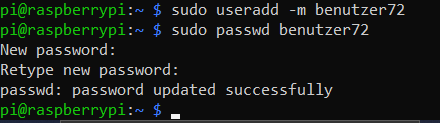
\includegraphics[scale=1]{Bilder/useradd_benutzer72.png}
        \caption{Anlage und Konfiguration des Benutzers \glqq benutzer72\grqq}\label{pic:useradd_72}
    \end{center}
\end{figure}

\begin{figure}[H]
    \begin{center}
        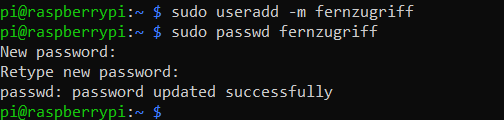
\includegraphics[scale=1]{Bilder/useradd_fernzugriff.png}
        \caption{Anlage und Konfiguration des Benutzers \glqq fernzugriff\grqq}\label{pic:useradd_fernzugriff}
    \end{center}
\end{figure}

\begin{figure}[H]
    \begin{center}
        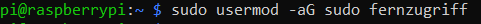
\includegraphics[scale=1]{Bilder/sudo_fernzugriff.png}
        \caption{Benutzer \glqq fernzugriff\grqq{} in die Gruppe sudo aufnehmen}\label{pic:usermod_fernzugriff}
    \end{center}
\end{figure}

\begin{figure}[H]
    \begin{center}
        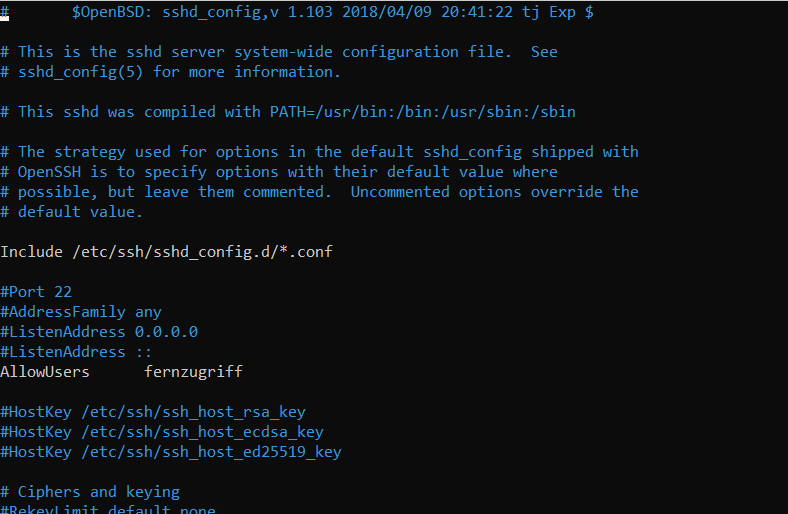
\includegraphics[scale=1]{Bilder/ssh_fernzugriff.png}
        \caption{Benutzer \glqq fernzugriff\grqq{} SSH-Rechte gewähren}\label{pic:ssh_fernzugriff}
    \end{center}
\end{figure}


\subsubsection{Konfiguration Netzwerk}




\subsubsection{Konfiguration Firewall}
\begin{figure}[H]
    \begin{center}
        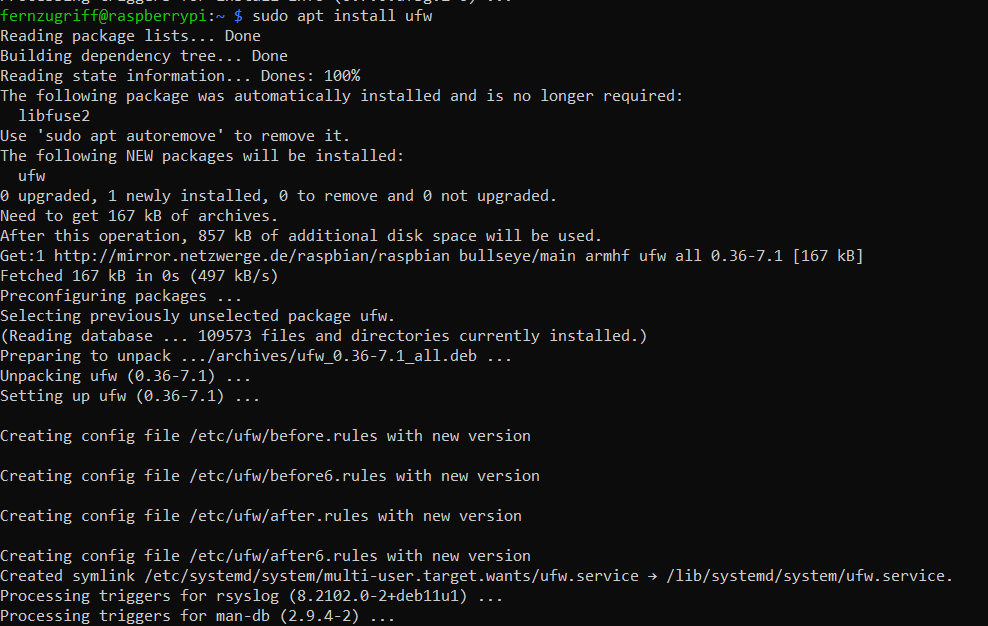
\includegraphics[scale=0.7]{Bilder/install_firewall.png}
        \caption{Installation der UFW Firewall}\label{pic:install_firewall}
    \end{center}
\end{figure}

\begin{figure}[H]
    \begin{center}
        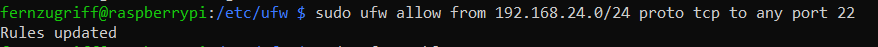
\includegraphics[scale=0.7]{Bilder/allow_ssh_from_network.png}
        \caption{SSH Port für gleiches Netzwerk öffnen}\label{pic:ssh_port_allow}
    \end{center}
\end{figure}

\begin{figure}[H]
    \begin{center}
        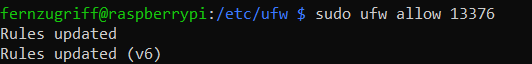
\includegraphics[scale=0.7]{Bilder/ufw_allow_api.png}
        \caption{Port der API für alle Netzwerke freischalten}\label{pic:api_port_allow}
    \end{center}
\end{figure}

\begin{figure}[H]
    \begin{center}
        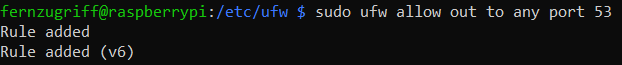
\includegraphics[scale=0.7]{Bilder/ufw_allow_out_dns.png}
        \caption{Ausgehende DNS Anfragen erlauben}\label{pic:dns_allow_out}
    \end{center}
\end{figure}

\begin{figure}[H]
    \begin{center}
        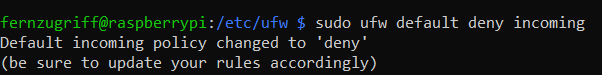
\includegraphics[scale=0.7]{Bilder/ufw_deny_all_incoming.png}
        \caption{Alle eingehenden Pakete ohne Regel verbieten}\label{pic:firewall_deny_default}
    \end{center}
\end{figure}

\begin{figure}[H]
    \begin{center}
        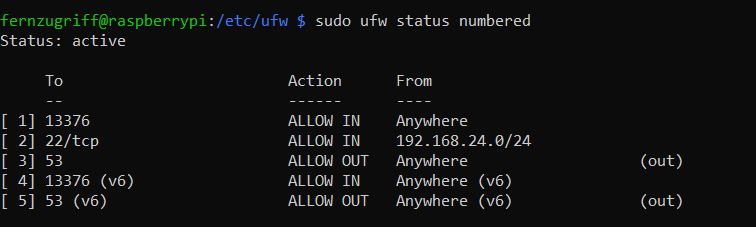
\includegraphics[scale=0.7]{Bilder/ufw_status_all_rules.png}
        \caption{Übersicht aller angelegten Regeln}\label{pic:firewall_status}
    \end{center}
\end{figure}





\subsection{Quellen}
\begin{small}

\end{small}
\end{document}